\documentclass[12pt]{article}
\usepackage[utf8]{inputenc}
\usepackage{graphicx}
\usepackage[a4paper,width=150mm,top=25mm,bottom=25mm]{geometry}
\title{

\\
{COS 301 Technology Requirements}
}

\author{Ctrl Alt Defeat}

\begin{document}

\begin{titlepage}
    \centering



    \vspace{2cm}
    \hrulefill\\
    \vspace{1cm}
    {\Huge\bfseries SRS Documentation v3.0}

    \vspace{1cm}

    {\Large Software Requirements Specification Document for\\Domain Pulse}\\
    \vspace{1cm}
    \hrulefill\\

    \vfill

    {\large Ctrl Alt Defeat}

    \vspace{1cm}

    {\large 2023/07/31}\\
    %    \vspace{1cm}
    %    \vspace{1cm}
    %    
\includegraphics[width=10cm]{../../Images/dpLogo.png}
    %    \vspace{1cm}\\
    %    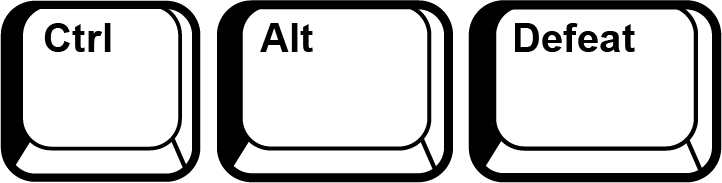
\includegraphics[width=6cm]{../../Images/cadLogo.png}

\end{titlepage}



\tableofcontents

\newpage

\section{Technology Requirements}

\subsection{Development Environment}
For development, our team members shall be developing within VS Code on Linux to ensure consistency within the produced code and testing of our software. Having all members using VS Code also allows for the use of software such as Live Share for collaborative development to improve efficiency within development.

\subsection{Version Control}
Git will be used for version control, using a clear and simple branching strategy that allows members to easily work on distinct components of our system while also allowing the reverting to previous versions as a 'fail-safe'. Meanwhile, GitHub will be used to host the Git repository.

\subsection{Programming Languages}
Within our team, many (if not all) members have a high proficiency in coding in Python. Python is considered one of the best programming languages for Machine Learning and data analysis, which are aspects on which our system will heavily rely. Therefore, Python is our programming language of choice.

\subsection{Frameworks and Libraries}
We have decided to use Django as our web framework for the creation of our app due to its simplicity, efficiency, and secure data transmission capabilities. Within our Django project, we will be utilizing Python's proficiency in data analysis and machine learning by using the powerful Vader and Grafana libraries, which allow us to perform sentiment analysis on text and visualize our data, respectively. For the front-end development, we will be using Angular due to its versatility and ability to create high-quality user interfaces.

\subsection{Database Systems}
For our database systems, we will be using MongoDB as a document-based NoSQL database for data collection of comments, posts, and other content related to user data. Additionally, PostgreSQL will be used as an SQL database for storing user profiles and authentication data for ease of access and querying.

\subsection{Testing and Quality Assurance Tools}
We will perform various forms of testing to ensure the quality of our software. For front-end testing, Cypress will be used, and for unit testing, we will utilize the built-in Unittest library of Python, which is recommended for Django.

\subsection{Deployment and Infrastructure}
For deployment, our clients have provided a Linux-based virtual machine where we can deploy our software. We will use one virtual machine for the testing environment and another for the production environment to ensure a separation of concerns. Additionally, a domain may be acquired for ease of customer access to the software.

\subsection{Collaboration and Communication Tools}
To ensure effective communication within our team, we have a private WhatsApp group for important announcements, a private Discord server for more specific announcements and discussions, and a GitHub Project Board to track work progress. For communication with our clients, we have set up a Slack workspace for quick communication.

\subsection{Security and Encryption}
Our system is secured using technologies such as Django's authentication system, which encrypts user data. We prioritize the use of POST over GET for more secure data transmission. Our virtual machine is protected by extensive firewalls to prevent foreign attacks, and access is restricted to authorized members of our team using SSH and private login details.

\subsection{Continuous Integration and Deployment Tools}
We will utilize CI/CD technologies such as Codecov and GitHub Actions to ensure thorough testing and checking before deployment. GitHub Actions will automate the building, testing, and deployment processes, while Codecov will provide insights into test results and failures. We have been provided with separate production and testing environments to deploy and check the application's functionality.

\end{document}